%%%%%%%%%%%%%%%%%%%%%%%%%%%%%%%%%%%%%%%%%
% Texas A&M University Physics Template
% This template has been downloaded from:
% http://www.LaTeXTemplates.com
%
% Modified by Joe Becker
%
% License:
% CC BY-NC-SA 3.0 (http://creativecommons.org/licenses/by-nc-sa/3.0/)
%
%%%%%%%%%%%%%%%%%%%%%%%%%%%%%%%%%%%%%%%%%

%----------------------------------------------------------------------------------------
%	PACKAGES AND THEMES
%----------------------------------------------------------------------------------------

\documentclass{beamer}

\mode<presentation> 

\usetheme{Madrid}
\usecolortheme{dolphin}
\usefonttheme{professionalfonts}

\setbeamertemplate{navigation symbols}{} 

\setbeamertemplate{footline}
{
\leavevmode%
\hbox{%
    \begin{beamercolorbox}[wd=.333333\paperwidth,ht=2.25ex,dp=1ex,center]{section in head/foot}%
        \usebeamerfont{author in head/foot}\insertshortauthor \ {(\insertshortinstitute)}
    \end{beamercolorbox}%
    \begin{beamercolorbox}[wd=.333333\paperwidth,ht=2.25ex,dp=1ex,center]{section in head/foot}%
        \usebeamerfont{title in head/foot}\insertshorttitle
    \end{beamercolorbox}%
    \begin{beamercolorbox}[wd=.333333\paperwidth,ht=2.25ex,dp=1ex,right]{section in head/foot}%
        \usebeamerfont{date in head/foot}\insertshortdate{}\hspace*{2em}
    \end{beamercolorbox}}%
    \vskip0pt%
}

\setbeamertemplate{frametitle}
{
    \begin{beamercolorbox}[sep=0.3cm,ht=1.8em,wd=\paperwidth]{frametitle}
        \vbox{}\vskip-0.0ex%
        \strut\insertframetitle\strut
        \hfill
        \vskip-2.8ex%
    \end{beamercolorbox}
}

\definecolor{maroon}{RGB}{25,25,180}

\setbeamercolor{title}{bg=maroon, fg=white}
\setbeamercolor{block title}{bg=maroon, fg=white}
\setbeamercolor{block body}{bg=maroon!05, fg=black}
\setbeamercolor{frametitle}{fg=maroon, bg=white}
\setbeamercolor{item}{fg=maroon}
\setbeamercolor{section in head/foot}{bg=maroon, fg=white}


\usepackage{graphicx}
\usepackage{booktabs}
\usepackage{textpos} 
\usepackage{media9}


%----------------------------------------------------------------------------------------
%	TITLE PAGE
%----------------------------------------------------------------------------------------

\title[Group Meeting]{Germanium Vacancy Diamond Zero Phonon Line Temperature Response}

\author[J. Becker]{Joe Becker}

\institute[Texas A\&M]{Texas A\&M Department of Physics and Astronomy

\medskip
\textit{jbecker@physics.tamu.edu} 
}

\date{January 26, 2017} 

\titlegraphic{
\includegraphics[height=1.5cm]{Images/TAMU_logo.png}}

%----------------------------------------------------------------------------------------
% PRESENTATION SLIDES
%----------------------------------------------------------------------------------------

\begin{document}
\setbeamertemplate{items}[circle]

\begin{frame}
\titlepage 
\end{frame}

\begin{frame}\frametitle{GeV Temperature Spectra}
    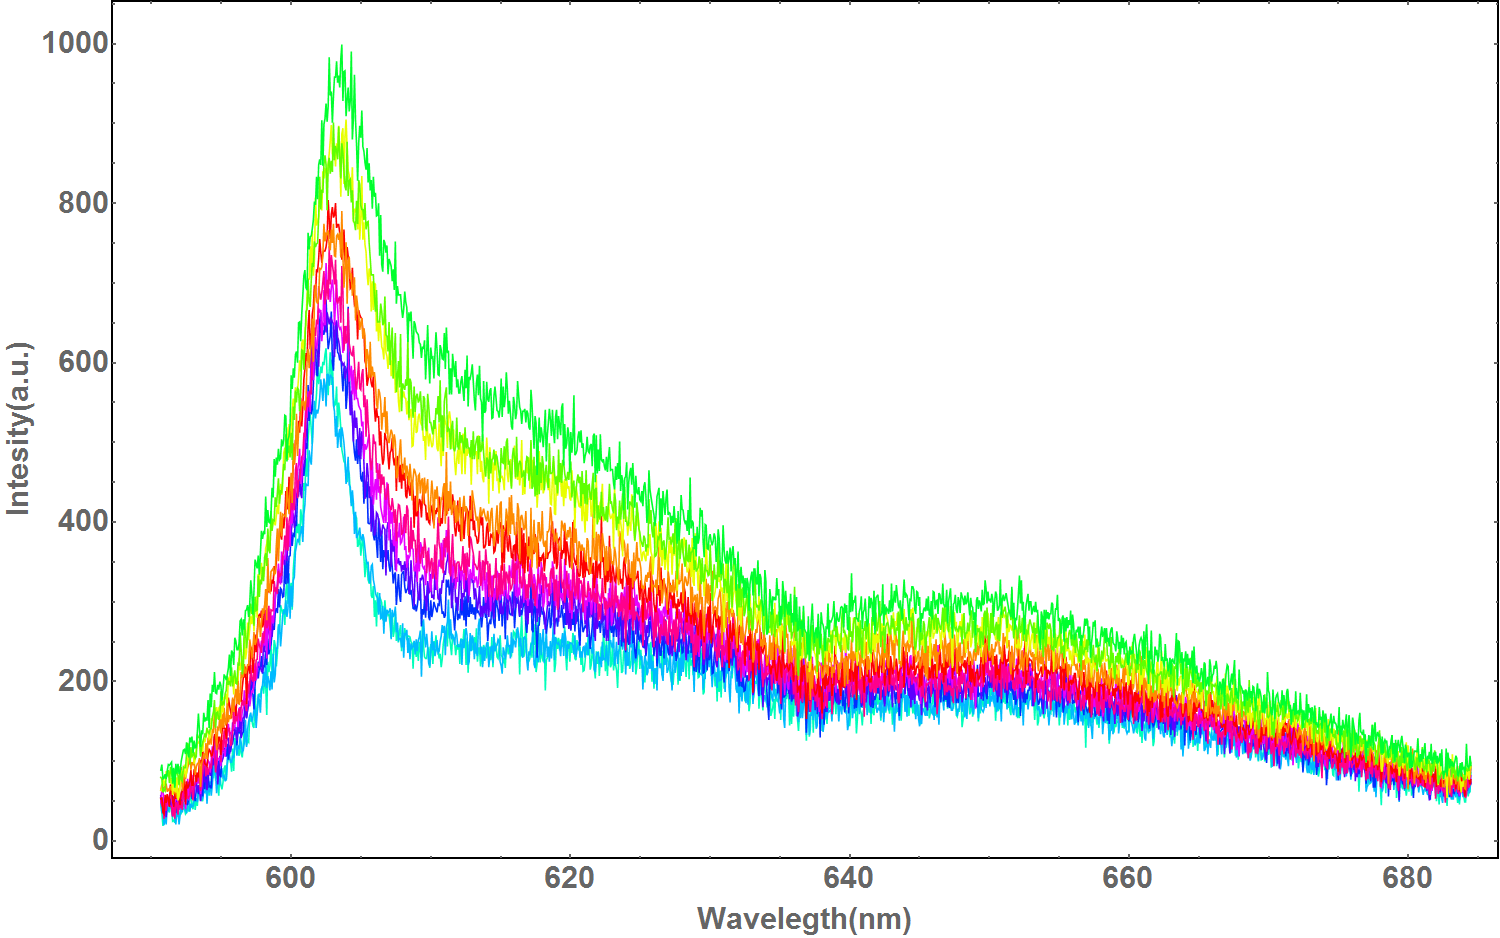
\includegraphics[width=1.0\textwidth]{Images/TempSpectrum.png}
\end{frame}

\begin{frame}\frametitle{300 K Spectrum Fit}
    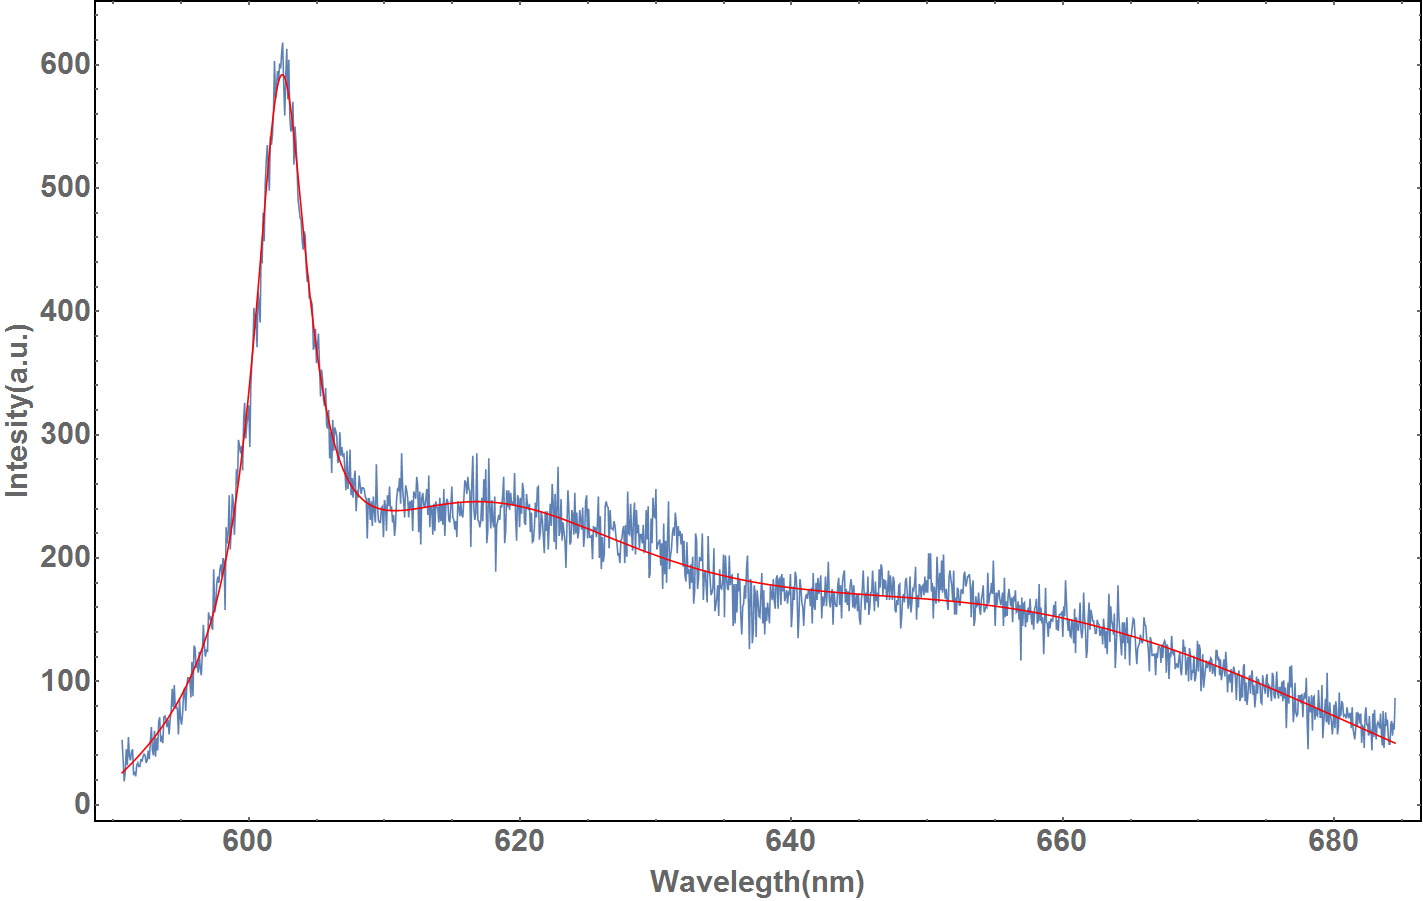
\includegraphics[width=0.95\textwidth]{Images/300KFit.png}

    Fit using 3 Lorentzian functions with an error function filter
\end{frame}

\begin{frame}\frametitle{ZPL Center Wavelength}
    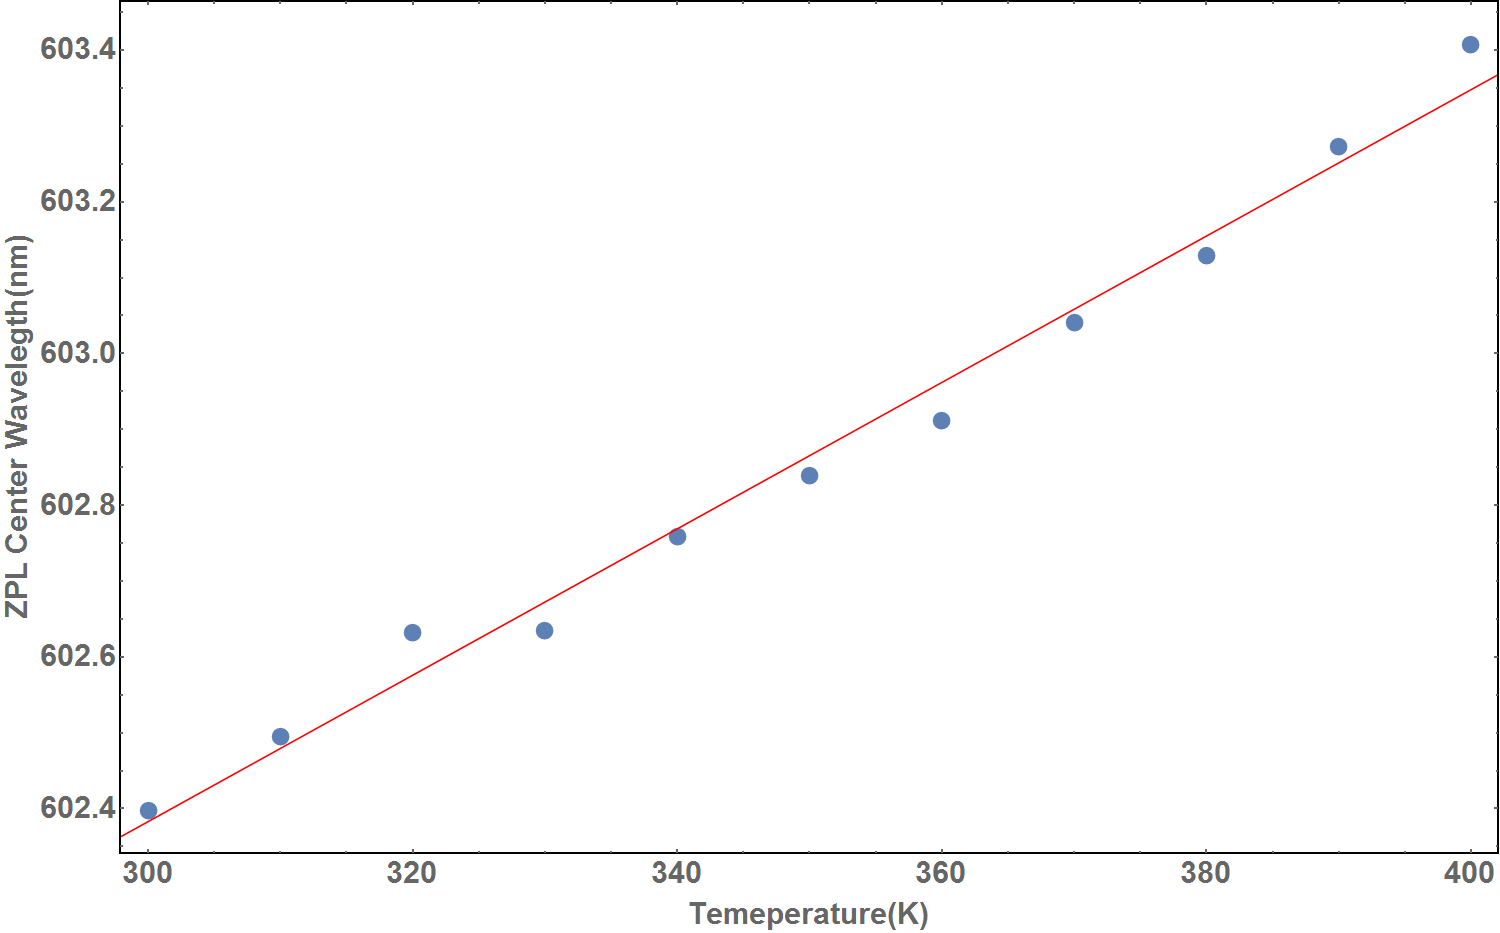
\includegraphics[width=0.95\textwidth]{Images/ZPFCenter.png}

    Fit: $y(x) = 599.488 + 0.00965032x$
\end{frame}

\begin{frame}\frametitle{ZPL Linewidth}
    \includegraphics[width=0.95\textwidth]{Images/ZPFLineWidth.png}

    Fit: $y(x) = -2.04259 + 0.0151333x$
\end{frame}

\begin{frame}\frametitle{ZPL Max Intensity}
    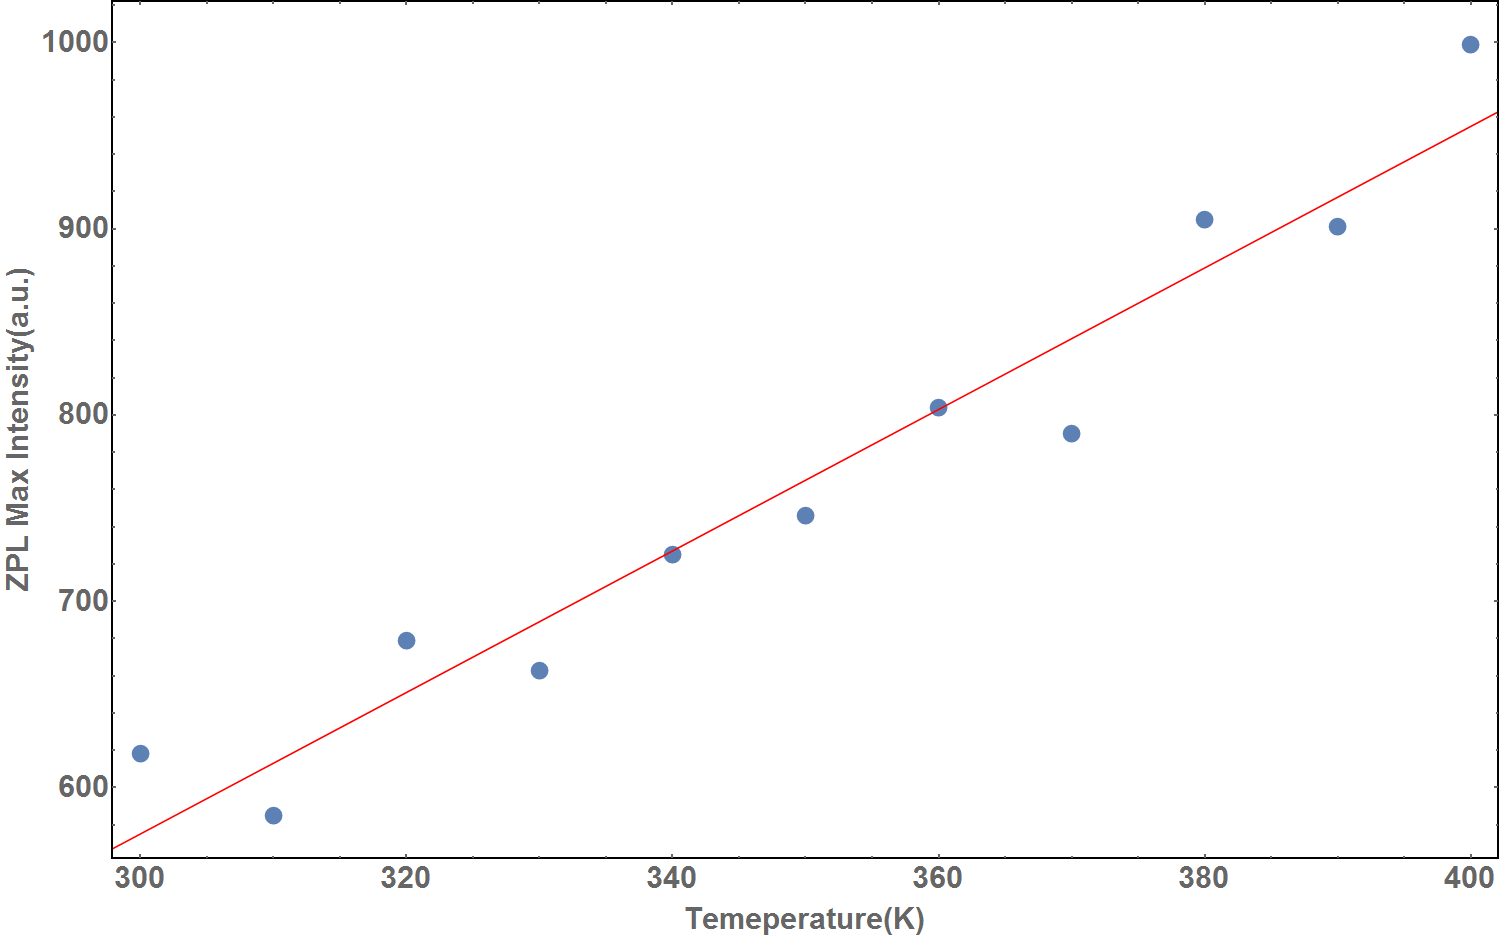
\includegraphics[width=0.95\textwidth]{Images/ZPFMaxIntensity.png}

    Fit: $y(x) = -565 + 3.8x$
\end{frame}
\end{document}

